\section{The audit of the saved model versions}
\label{sec:results}

The audit read every saved world-model and lift-model checkpoint of the
companion paper~\cite{rwm}: \rVersions{} versions (a configuration and seed),
\rVerM{} on M5, \rVerD{} on Dominick's and \rVerF{} on Frat, scored on
\rWindows{} version-windows. Most are development variants, so they differ in
many settings at once. No model was refitted or tuned. Table~\ref{tab:realpass}
gives the pass counts and Figure~\ref{fig:realchecks} every score.

\begin{table*}[t]\centering
\caption{\textbf{No version passed every check on M5 or Dominick's.} Pass counts
by check and data set, over version-windows (a check counted only where it
applies: C3 needs two or more seeds, C6 a LightGBM run on the same window).
Thresholds in Table~\ref{tab:thresholds}.}\label{tab:realpass}
\footnotesize\setlength{\tabcolsep}{6pt}\input{generated/tab_real_pass}\end{table*}

\begin{figure*}[t]\centering
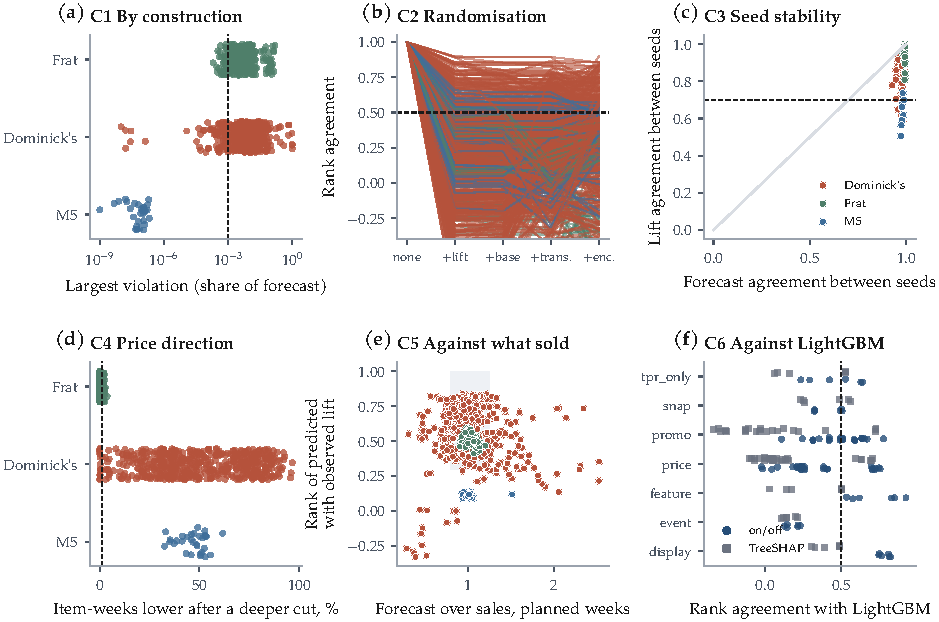
\includegraphics[width=\textwidth]{figs/fig_real_checks.pdf}
\caption{\textbf{The explanations agreed with themselves across seeds on
Dominick's and Frat, failed the price-direction check on Dominick's and M5,
and agreed with LightGBM only on Frat.} One point per version-window, coloured
by data set; dashed lines: pass thresholds. \textbf{(a)} C1, the largest
violation of the construction properties as a share of the largest forecast.
\textbf{(b)} C2, rank agreement of the total lift with the original as the lift
readout, baseline readout, transition and encoder are re-initialised in turn.
\textbf{(c)} C3, agreement of lifts between seeds against agreement of
forecasts. \textbf{(d)} C4, the share of item-weeks forecast lower after a
deeper price cut. \textbf{(e)} C5, forecast over sales and rank of predicted
with observed lift on planned item-weeks; shaded: the pass region. \textbf{(f)}
C6, rank agreement with LightGBM's on/off contributions (circles) and TreeSHAP
values (squares), by lever.}\label{fig:realchecks}
\end{figure*}

\paragraph{No version passes every check on M5 or Dominick's}
On Frat \rAllF{} of \rWinF{} version-windows pass every check that applies;
on M5 and Dominick's none do. The checks fail for different reasons on each
data set, and two of them, C1 and C4, needed a diagnosis before they could be
read. C4 was rerun on \dRuns{} saved runs (\dWindows{} windows) chosen by a rule
fixed before the rerun (\texttt{docs/PAPER2\_PLAN.md}, 17 October), and C1 was
traced for every audited configuration (18 October); both diagnoses are
reported as added after the results.

\paragraph{C1: the parts add up, and every failure traces to what ``nothing planned'' means}
In every version baseline plus lift equals the forecast (largest violation
\rCaPartsMax{} of the largest forecast), and the baseline moves with the plan by
at most \rCaBaseMax\% of it. The lift when nothing is planned passes on all
\rVerM{} M5 versions, but only on \rPassDCa{} Dominick's and \rPassFCa{} Frat
version-windows, with a median violation of \rMedDCaPct\% and \rMedFCaPct\% of
the largest forecast. These failures come from two definitions of nothing
planned. The audit's plan turns the levers off and sets each price to the
series' highest price over the last 12 training periods, keeping the planned
price where the series has none. Each model has its own plan: the levers off
and its own regular price, taken over its history window, from a recorded or a
held regular price where its configuration says so, and otherwise the series'
mean price over that window, or 1.0 where the window records no price. Given
the model's own plan, the lift is zero for every series with history, because
the plan path and the nothing-planned path then receive identical inputs; on
saved Frat runs the violation fell from 0.04\% to 0.09\% of the largest
forecast under the audit's plan to under $10^{-7}$ under the model's.

Whether the two plans differ depends on the data and the settings, not on the
fitted weights, so we compared them for every audited configuration and window
(\cIfN{} of the \cIfOf{} version-windows; \texttt{scripts/c1\_interface.py},
added after the results). They differ in \cIfAnyD{} Dominick's, \cIfAnyF{}
Frat and \cIfAnyM{} M5 version-windows (M5 checked on three of its ten
stores, for memory), on a median of \cIfMedD\% of
series-periods on Dominick's and \cIfMedF\% on Frat. Every one of the
\cIfFailN{} version-windows that fail C1 has a difference; all \cIfSameN{} in
which the plans agree pass, with violations no larger than \cIfSameMaxCa{} of
the largest forecast; \cIfDiffPass{} with a difference still pass, where the
series affected carry little lift. Of the series-periods that differ, \cIfShareNoReg\% are
series with no price in the audit's last 12 periods, where the model uses its
fallback (a price of 1.0 in \cIfShareOne\% of all differing series-periods);
\cIfShareRule\% are configurations whose regular price comes from a held or a
recorded price; and \cIfShareNew\% are new items, whose baseline borrows several
other series' regular prices, so that no single plan matches it. Where the two
prices differ they are a median \cIfGap{} times apart.

C1 under the audit's plan therefore measures the interface between the audit
and the model, not a broken decomposition. It also shows a fault a merchant
would care about: for an item with no recent price, the model's baseline is
computed at a price nobody would plan, and the lift absorbs the difference. The
audit's C1 scores and pass counts are reported unchanged in
Table~\ref{tab:realpass} and the main test.

\paragraph{C2 and C3: the lifts depend on what was learned, and agree across seeds where the data are rich}
After the lift readout is re-initialised the lifts' rank agreement with the
original falls below 0.5 in \rPassDCb{} Dominick's, \rPassFCb{} Frat and
\rPassMCb{} M5 version-windows (medians \rMedDCb, \rMedFCb{} and \rMedMCb), so
the lifts mostly depend on what the readout learned; in the known-answer study
the same check did not separate correct models from broken ones
(\S\ref{sec:known}), so a pass here says little. Seeds agree on the lifts with a
median rank agreement of \rStabLiftF{} on Frat and \rStabLiftD{} on Dominick's,
but only \rStabLiftM{} on M5, against \rStabFcM{} to \rStabFcF{} for the
forecasts themselves on every data set. On M5, where prices rarely change and
the plan is mostly event and SNAP days, fits that agree on the forecast disagree
on how much of it the plan explains; \rPassMCc{} M5 version-windows pass C3.

\paragraph{C4: on Dominick's and M5 a deeper price cut often lowers the forecast}
A deeper cut gives a forecast lower by more than 0.1\% in a median of
\rMedDCdPct\% of Dominick's and \rMedMCdPct\% of M5 item-weeks, against
\rMedFCdPct\% on Frat; \rPassDCd{} Dominick's and \rPassMCd{} M5 version-windows
pass. The diagnosis rules out the two simple explanations. Cutting only a random
tenth of series, so that other items' cuts barely enter, gives the same share
(median \dCdTenthD\% against \dCdAllD\% on Dominick's, \dCdTenthM\% against
\dCdAllM\% on M5). And the drops are not small: in a median of \dCdBigD\% of
Dominick's and \dCdBigM\% of M5 item-weeks the forecast falls by more than 5\%,
and the share is already \dCdFiveD\% and \dCdFiveM\% at the first 5\% cut. On
Frat \dCdBigF\% of item-weeks fall by more than 5\%. On Dominick's and M5 these
models' forecast fell after a deeper cut in about half the item-weeks or more,
and no accuracy score showed it. (The rerun runs, chosen partly for large C1
violations, show higher shares than the full audit on Dominick's.)

\paragraph{C5 and C6: agreement with sales and with LightGBM}
On planned item-weeks the forecast is close to sales in total on every data set
(median bias \rMedDCeBias, \rMedFCeBias{} and \rMedMCeBias), and the rank
agreement of predicted with observed lift is \rMedDCeRank{} on Dominick's and
\rMedFCeRank{} on Frat but \rMedMCeRank{} on M5 (event days \rCeMevent, SNAP days
\rCeMsnap), so no M5 version passes C5. Agreement with LightGBM's total lift
passes on Frat (median \rMedFCf) and mostly fails on Dominick's (\rMedDCf) and
M5 (\rMedMCf). Lever by lever, the models' promotion contributions on Dominick's agree with
LightGBM's on/off contributions (median rank agreement \rAgDpromoOn) but not
with its TreeSHAP values (\rAgDpromoShap); on Frat they agree with both
(\rAgFpromoOn{} and \rAgFpromoShap). Which attribution of LightGBM one compares
with can change the verdict.

\paragraph{C7: both models state a larger price response than the one measured}
Over the \rZEpisodes{} scored zone price episodes, the pooled slope of the stated
response on the price deviation is \rZSlopeWorld{} for the world model (95\%
interval \rZSlopeWorldLo{} to \rZSlopeWorldHi) and \rZSlopeLgb{} for LightGBM
(\rZSlopeLgbLo{} to \rZSlopeLgbHi), against \rZSlopeMeas{} (\rZSlopeMeasLo{} to
\rZSlopeMeasHi) measured over the same eight weeks and about $-0.3$ in the
chain's own experiments (Figure~\ref{fig:realc7}). Both models state roughly
twice the measured response, though the measured interval is wide and overlaps
both, the pattern the known-answer study produced when a
model answers a question about the regular price with what it learned from
temporary cuts (\S\ref{sec:known}). The measured interval is wide and overlaps
the world model's, so these episodes do not exclude the world model's slope;
both models' intervals lie below the $-0.3$ the experiments implied. Per episode,
the world model's stated response falls inside the measured interval in
\rZWorldInside{} of \rZEpisodes{} episodes and LightGBM's in \rZLgbInside, but
those intervals are too narrow to trust (\S\ref{sec:zones}); the stated response
has the expected sign in \rZWorldSign{} and \rZLgbSign{} episodes, the measured
one in \rZMeasuredSign.

\begin{figure*}[t]\centering
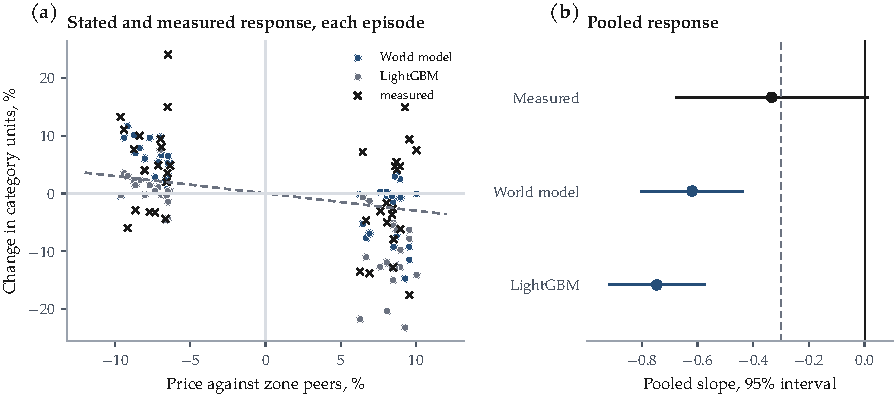
\includegraphics[width=\textwidth]{figs/fig_real_c7.pdf}
\caption{\textbf{The world model and LightGBM state about twice the measured
response to a regular price change; the measured interval is wide.} \textbf{(a)} For each scored Dominick's
zone price episode, the store's price against its zone peers and the change in
its category units over the first eight weeks: stated by the world model and
LightGBM, each fitted up to the week before the episode, and measured by
difference in differences; dashed: an elasticity of $-0.3$. \textbf{(b)} Pooled
slope across episodes with a 95\% interval robust to unequal variances.}
\label{fig:realc7}
\end{figure*}

\paragraph{The main test: on these versions, passing more checks did not clearly go with forecasting better}
On the unit fixed before any result, a version and window, the correlation
across version-windows between the number of checks passed and item-by-store
WRMSSE is \rRhoPassedM{} on M5, \rRhoPassedD{} on Dominick's and \rRhoPassedF{}
on Frat; pooled, \rRhoPassedPool{} (permutation $p = \rPPassed$;
Table~\ref{tab:realmain}). Averaged over each version's windows the pooled
correlation is \rRhoPassedPoolV{} ($p = \rPPassedV$). The answer moves with the
unit, and neither permutation keeps the dependence in these data: versions that
share a configuration, configurations that differ in one setting, and versions
scored on the same window are not independent, and a window that is easier and
passes C1 and C4 less often (the second Frat window) enters the
version-window correlation as a relation between checks and error.

We therefore reran the test, as an analysis added after the results, on
comparisons that hold the data and the window fixed. Seeds of a configuration
are averaged, so a configuration counts once per window. Configurations scored
on the same series and windows form a set (\rWwData{} sets with at least four
configurations, \rWwConfigs{} configurations in all); within each set and
window the Spearman correlation across configurations is taken, and the
correlations are pooled weighted by the number of configurations. The
permutation reassigns whole configurations, with their scores in every window,
within each set, and the interval comes from resampling configurations within
each set. No M5 set has four configurations, so M5 drops out. The pooled
correlation is \rWwRho{} (95\% interval \rWwLo{} to \rWwHi, $p = \rWwP$):
\rWwRhoD{} on Dominick's and \rWwRhoF{} on Frat. With C5 left out it is
\rWwNoCeRho{} (\rWwNoCeLo{} to \rWwNoCeHi, $p = \rWwNoCeP$), and with C1 and C5
left out \rWwNoCaCeRho{} (\rWwNoCaCeLo{} to \rWwNoCaCeHi, $p = \rWwNoCaCeP$).
C5 compares the forecast with sales over the same baseline and so shares
information with accuracy; on the unit fixed in advance it is the check most
strongly related to accuracy (rank of predicted with observed lift
\rRhoCeRankPool, bias \rRhoCeBiasPool).

What these data support is narrow. On these saved versions, configurations
compared on the same data and window that passed more checks did not clearly
forecast better or worse. The intervals run from about $-0.25$ to $0.12$: they
exclude a strong relation in either direction, not a weak one.
They do not show that faithfulness and accuracy are unrelated in general: the
versions are development variants of two model families, the checks measure
faithfulness only in part, and a stronger relation could hold across more
different models.

\begin{table*}[t]\centering
\caption{\textbf{Across versions, the number of checks passed was not clearly
related to accuracy; the check that was, C5, shares information with
accuracy.} Spearman correlation between each score and item-by-store WRMSSE
(negative: higher scores go with lower error), within each data set and pooled
by permutation within data set (10,000 permutations). Left: over
version-windows, the unit fixed in advance. Right: over versions, the mean over
each version's windows. Both permutations treat their units as independent; the test that holds the data and window fixed and keeps the dependence between related configurations is in the text. $^\dagger$Added after the results.}\label{tab:realmain}
\footnotesize\setlength{\tabcolsep}{6pt}\input{generated/tab_real_main}\end{table*}

\begin{figure*}[t]\centering
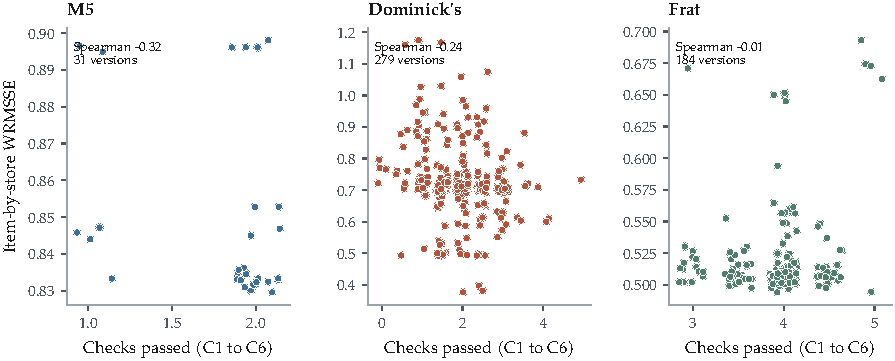
\includegraphics[width=\textwidth]{figs/fig_real_main.pdf}
\caption{\textbf{Checks passed against accuracy, one point per version.}
Item-by-store WRMSSE (lower is better) against the mean number of checks passed
over the version's windows, with the Spearman correlation within each data
set.}\label{fig:realmain}
\end{figure*}
